\documentclass[a6paper,10pt]{article}
%\usepackage[T1]{fontenc}
\usepackage[british]{babel}
\usepackage[utf8]{inputenc}
\usepackage{float, graphicx,amsmath,amsfonts,cite,enumerate,tabularx}
\usepackage[final]{pdfpages}
\usepackage{wrapfig}
\usepackage[margin=0.3in]{geometry}
\usepackage{../sidspaltHack}
\usepackage[framed,numbered,autolinebreaks,useliterate]{mcode}
\usepackage{../digital}


\setlength{\oddsidemargin}{-0.37in}
\setlength{\textwidth}{215pt}

\pagestyle{empty}
\begin{document}
\nysida{9}{1}
\noindent
\chaptertitle{I$\iota$}{Torra visor}
\begin{center}
\songtitle{$\iota1$}{Système International} 
\mel{Studentsången}
\end{center}
\vspace{-10pt}
\begin{table}[!h]
\begin{tabularx}{0.85\textwidth}{X X X X X}
W&kg&m&Wb&s
\vspace{3pt} \\
$\Omega$m&T&A&rad
\vspace{3pt} \\
Cd&S&N&s
\vspace{3pt} \\
$\Omega$A&m&Lx&dB
\vspace{3pt} \\
$^{\circ}$C&W/m$^2$ &
\vspace{5pt} \\
J/kg&H&V&C
\vspace{3pt} \\
kg/m$^3$ & mol
\vspace{3pt} \\
m/s$^2$&m/s$^2$&F!
\end{tabularx}
\auth{Skriven till Sångartäfvlan -75\\ av Anders Skog F-75}
\end{table}
\begin{center}
\songtitle{$\iota2$}{Integralkalkylens fader} 
\footnotesize SF1602 Differential- och integralkalkyl II\\
\mel{Sveriges fana}
\end{center}
\small Integralkalkylens fader, \\
G W Leibniz hette han. \\
Han blev trött på att skriva rader \\
av plustecken efter varann. 
\vspace{5pt}\\
Så han tänkte: \\
"Das Wort Summe, \\
es beginnt ja mit ein S". \\
Och han sade, \\
och han gjorde \\
integrationssymbolen av sitt S. 
\newpage
\setlength{\oddsidemargin}{-0.47in}
\noindent
Integralkalkylens fader \\
fick idén för länge se'n. \\
Den elfte uti november \\
sextonhudra-sjuttifem. \\
Se'n det året, \\
se'n den dagen, \\
vi skriver det tecknet så. \\
Och vi räknar \\
och kalkylerar, \\
integralens tecken kan man lita på. 
\vspace{5pt} \\
Och idag vi tecknet hylla. \\
Det löser alla problem. \\
Det lyckas vår fritid fylla \\
med dx och med dt:n. \\
Ja, må det leva. \\
Ja, må det leva, \\
i många hundrade år. \\
Så att våra barn \\
och våra barnbarn \\
integralens tecken lära får. 
\auth{Skriven till integralens\\ 300-årsdag 1975-11-11.}
\vspace{-10pt}
\begin{figure}[!h]
\hspace{30pt}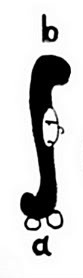
\includegraphics[width=0.15\textwidth]{integral.jpg}
\end{figure}

\nysida{9}{3}
\setlength{\oddsidemargin}{-0.37in}
\noindent
\begin{center}
\songtitle{$\iota3$}{GG-visan} 
\footnotesize5A1203 Fysik, grundkurs del I\\
\mel{Jag är ett litet ylle}
\end{center}
Jag heter Göran Grimvall, W pdV Vdp. \\
Med världens bästa infall, W pdV Vdp. \\
Jag lär ut termodynamik \\
och har problem i Ny Teknik. \\
Grimvall, Grimvall, \\
Grimvall på dig, Grimvall-freak. 
\vspace{5pt} \\
I julas ringde Platen, W pdV Vdp. \\
Precis efter julmaten, W pdV Vdp. \\
Hur kunde han störa då, den token, \\
jag tittade ju på Djungelboken. \\
Grimvall, Grimvall, \\
Grimvall på dig, Grimvall-snoken. 
\vspace{5pt} \\
Jag var student på Chalmers, W pdV Vdp. \\
Det här blir blott en halv vers, W pdV Vdp. 
\vspace{5pt} \\
Jag satt i kommissionen, W pdV Vdp. \\
För ubåtsinvasionen, W pdV Vdp. \\
Jag springer efter skärmar när \\
jag inte plockar svamp och bär. 
\vspace{5pt} \\
Grimvall, Grimvall,\\
 oj... nu sitter Grimvall där! 
\auth{n$\emptyset$llespexet 1999}

\nysida{9}{4}
\setlength{\oddsidemargin}{-0.47in}
\noindent
\begin{center}
\songtitle{$\iota4$}{Öl sex} 
\footnotesize SI1140 Vektoranalys\\
\mel{Med en enkel tulipan}
\end{center}
En liten enkel integral, \\
uti ett Vektor III-tal. \\
Ni har besväret, \\
ni har besväret, att derivera. 
\vspace{5pt} \\
Först tar en Stokes' sats däruppå, \\
så blir det så enkelt så. \\
Att integralen, \\
att integralen, evaluera. 
\vspace{5pt} \\
Och rotationen den integreras \\
sen över ytan utav en boll. \\
Och koordinaterna transformeras \\
så integranden blir bara noll. 
\vspace{5pt} \\
En liten enkel integral, \\
uti ett Vektor III-tal. \\
Kan va' så jävlig \\
att en ej hinner med något mera. 
\auth{F-CTH}
\begin{figure}[!h]
\hspace{120pt}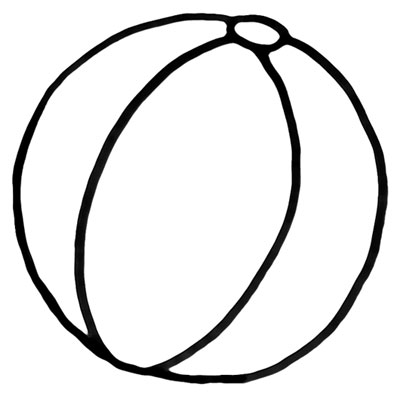
\includegraphics[width=0.3\textwidth]{boll.jpg}
\end{figure}

\nysida{9}{5}
\setlength{\oddsidemargin}{-0.37in}
\noindent
\begin{center}
\songtitle{$\iota5$}{The BASIC song} 
\footnotesize DD1346 Programkonstruktion\\
\mel{Mors lilla Olle}
\textit{Radnumren sjungs ej!}
\end{center}
10 LET oss nu fatta i våra glas\\
 20 INPUT en klunk utav det som där has\\
 30 IF du fått nog THEN till 50 min vän\\
 40 ELSE GOTO-baka till 10 igen\\
 50 END
\vspace{30pt}
\begin{center}
\songtitle{$\iota6$}{Mors lilla dator} 
\footnotesize DD1345 Grundläggande datalogi\\
\mel{Mors lilla Olle}
\end{center}
Mors lilla dator åt skogen gick, \\
mitt i programmet sade det klick. \\
Svart bidde skärmen och minnet försvann, \\
den informationen kan ingen få fram. 
\vspace{5pt} \\
Brummeli-brum vad brummar där? \\
Det sprakar och gnistrar, ett jordfel det är!! \\
Blixtar blå från burken det slå, \\
synd att jag här nu ensam stå. 
\vspace{5pt} \\
Hyscheli-hysch vad prasslar här? \\
Fram väller pappret ur printern där! \\
Den har fått nippran av tecken så små, \\
jag tror att jag snart hemåt skall gå. 

\nysida{9}{7}
\setlength{\oddsidemargin}{-0.47in}
\noindent
\begin{center}
\songtitle{$\iota7$}{Tentamenssång} 
\mel{Stockholmsmelodi}
\end{center}
Se hur hela Teknis går i vånda. \\
Snart så kommer tentaperiod. \\
Mek på fredag sedan Funk på måndag. \\
Det är så att en kan gråta blod. 
\vspace{5pt} \\
Vad har jag gjort hela långa våren, \\
när jag skulle pluggat och stått i. \\
Jag har bara druckit öl på kåren, \\
men det kan en inte tenta i. 
\vspace{5pt} \\
Se så många stackars teknologer. \\
Transpirerar i en kvalmig sal. \\
Grubblar planlöst över svåra frågor. \\
Suckar, deppar åt en massa tal. 
\vspace{5pt} \\
Skriver formler, söker kombinera, \\
för att få ihop en ekvation. \\
Sedan kan de ilsket konstatera, \\
att de ej fått rätt på dimension. 

\begin{flushright}
\large
\begin{align*}
&m\ddot{x} + c\dot{x} + kx = mg \\
&\dot{x} = A\omega_n\cos{\omega_nt}\\
&\tau = 2\pi/\omega_n\\
&\omega_n = \sqrt{k/m}
\end{align*}
\end{flushright}

\nysida{9}{8}
\setlength{\oddsidemargin}{-0.37in}
\noindent
\begin{center}
\songtitle{$\iota8$}{ODE till en husvagn} 
\footnotesize SG1130 Mekanik, baskurs\\
\mel{Husvagn}
\end{center}
Vi har ägnat våren åt en kurs i mekanik, \\
prickar, streck och pilar och en massa dynamik. \\
Vi har haft svårt att fatta vad en svängning innebär\\ 
men äntligen har vi förstått vad Newtons lagar lär...
\vspace{5pt} \\
En ska ha husvagn, som sitter fastspänd i en båt. \\
En ska ha husvagn, som sedan sjunker och blir våt. \\
En ska ha husvagn, som först är odämpad och fri. \\
En ska ha husvagn, nu så fattar vi! 
\vspace{5pt} \\
En tänker sig en vagn med massan $m$ och så en fjäder \\
som står på däcket på en båt som seglar i hårt väder. \\
När båten gungar skapas det en svängningsekvation, \\
och vattnet som sen strömmar in ger stark viskös friktion. 
\vspace{5pt} \\
En ska ha husvagn, då kommer en att räkna rätt. \\
En ska ha husvagn, för då kan resten inses lätt. \\
En ska ha husvagn, det är ett bra svängningssystem. \\
En ska ha husvagn i sina problem! 
\vspace{5pt} \\
$m \ddot{x} + c \dot{x} + k x$ är $m g$ \\
$\dot{x}$ är $A \omega_n \cos \omega_n t$ \\
$\tau$ är lika med $2\pi$ genom $\omega_n$, \\
där $\omega_n$ är roten ur $k$ genom $m$.
\vspace{5pt} \\
En ska ha husvagn, det är en bild som är konkret. \\
En ska ha husvagn, men för en hög viskositet \\
ska man ha honung, det ger ett $\zeta$ som är högt. \\
En ska ha honung, för det är kladdigt, mjukt och sött! 
\auth{Första Fulölfesten, 2000}

\nysida{9}{9}
\setlength{\oddsidemargin}{-0.47in}
\noindent
\begin{center}
\songtitle{$\iota9$}{Matlab} 
\footnotesize DN1240 Numeriska metoder, grundkurs II\\
\mel{Husvagn}
\end{center}
Jag har prövat nästan allt som finns att pröva på:\\
Kulram, fingrar, räknesticka, tärning eller så.\\
Jag har kalkylerat på de konstigaste sätt\\
men nu så har jag kommit på hur en ska räkna rätt.
\vspace{5pt} \\
En ska ha \mcode{MATLAB}, då är kalkylen redan klar.\\
En ska ha \mcode{MATLAB}, det har jag sett att andra har.\\
En ska ha \mcode{MATLAB}, det är min livsfilosofi.\\
En ska ha \mcode{MATLAB}, för då blir en fri.
\vspace{5pt} \\
I många år så var jag inte alls så särskilt lärd.\\
Jag visste ej vad som vänta’ mig i denna stora värld.\\
Men sedan jag till NADA kom, och ända sedan dess\\
så har jag funnit livets stora lyxdelikatess.
\vspace{5pt} \\
En ska ha \mcode{MATLAB}, så att en slipper tänka alls.\\
En ska ha \mcode{MATLAB}, ja, då går allting som en vals.\\
En ska ha \mcode{MATLAB}, det bygger på nån slags logik.\\
En ska ha \mcode{MATLAB}, för då blir en rik.
\vspace{5pt} \\
5 minuter mekanik, 5 minuter statfys,\\
5 minuter kvantfysik, 5 minuter analys,\\
5 minuter fråga propp, 5 minuter kolla opp,\\
5 minuter tänka själv och sedan tar det stopp.
\vspace{5pt} \\
En ska ha \mcode{MATLAB}, och datasalens friska luft.\\
En ska ha \mcode{MATLAB}, det tycker studenterna är tufft.\\
En ska ha \mcode{MATLAB}, när Ryssen kommer med sitt MIG.\\
En ska ha \mcode{MATLAB}, då vinner en i krig.
\auth{Uppsala teknologers sångbok}

\nysida{9}{10}
\setlength{\oddsidemargin}{-0.37in}
\noindent
\begin{center}
\songtitle{$\iota10$}{Hållfvisa} 
\footnotesize SE1055 Hållfasthetslära, grundkurs F\\
\mel{Mors lilla Olle}
\end{center}
Mohrs lilla cirkel i skogen kröp. \\
Gränslast på axeln och skjuvning i blick. \\
Ytorna små utav tryck äro blå. \\
Tänk om jag slapp att få flyta ändå. 
\vspace{5pt} \\
Brumelibrum, vem stöter där? \\
Knakar, en dislokation visst det är. \\
$\sigma$ den ökar och cirkeln blir krökt: \\
Hör du, jag tror att du spänner för högt. 
\vspace{5pt} \\
Hooke fick nu se dem, gav till ett skri. \\
Linjen försvann, nu är leken förbi. \\
Å varför skrämde du undan min vän? \\
Mohr lilla bed honom käla igen. 
\auth{Mikael Ros 1975}

\begin{figure}[!h]
\centering
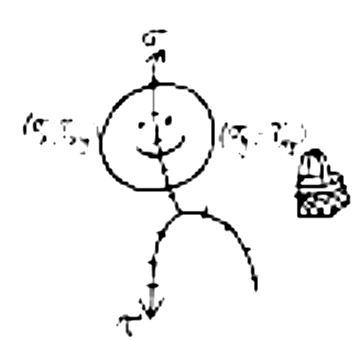
\includegraphics[width=0.4\textwidth]{Hallfgubbe.png}
\end{figure}

\nysida{9}{11}
\setlength{\oddsidemargin}{-0.47in}
\noindent
\begin{center}
\songtitle{$\iota11$}{Elämnenas lov} 
\footnotesize EI1240 Teoretisk elektroteknik\\
\mel{Trink, Trink}
\end{center}
Ström, ström, vi vill ha ström. \\
Det är vår senaste dröm. \\
Ström, ström, vi vill ha ström. \\
Det är vår senaste dröm. 
\vspace{5pt} \\
Shunta din MOS \\
och bottna din FET \\
och ge mig en puls utav det. \\
Slut upp i kampen för Elmät och TET. \\
Ström är det bästa vi vet! 
\vspace{20pt} 
\begin{center}
\songtitle{$\iota12$a}{O hemska lab} 
\footnotesize2B1507 Halvledarelektronik\\
\mel{O Helga Natt}
\end{center}
O hemska lab, o grymma kval imorgon. \\
Här sitter jag och förstår ingenting. \\
Hela mitt inre fylls utav ett motstånd \\
emot eländig elektrisk mätteknik. 
\vspace{5pt} \\
Jag skulle nog behöva lite ledning, \\
Här räcker inte min kapacitans. 
\vspace{5pt} \\
Kondensatorer och felvända dioder. \\
O hemska lab, nu vill jag koppla af. \\
O hemska lab, ty detta blir min graf! 
\auth{Sångartäfvlan 1992}

\newpage
\setlength{\oddsidemargin}{-0.37in}
\noindent

\begin{center}
\songtitle{$\iota12$b}{O hemska lab} 
\footnotesize DD1331 Grundläggande programmering\\
\mel{O Helga Natt}
\end{center}
O hemska lab, o grymma kval imorgon. \\
Här sitter jag och förstår ingenting. \\
Hela programmet är fyllt utav funktioner\\
som innehåller en himla massa fel. 
\vspace{5pt} \\
Pekare som inte har nån riktning, \\
oändliga loopar, oj vad jag blir sträng!
\vspace{5pt} \\
Åh, kompilera, hur ska det här fungera? \\
O hemska lab, nu vill jag logga ut. \\
O hemska lab, ty detta blir mitt slut! 

\begin{center}
\songtitle{$\iota12$c}{O hemska lab} 
\footnotesize SI1121 Termodynamik\\
\mel{O Helga Natt}
\end{center}
O hemska lab, o fasliga arbete. \\
Det pumpar bort all min inre energi. \\
Denna process förvärrar nog mitt tillstånd, \\
jag är helt fast, med utvägen medelfri. 
\vspace{5pt} \\
Det känns som att jag håller på att kvävas, \\
ty jag har inte hunnit värma upp. 
\vspace{5pt} \\
Mystiska lådor och vätske-värmepumpar. \\
O hemska lab, mitt lärande blir svalt. \\
O hemska lab, det känns ej idealt! 
\auth{Adam Erlandsson, F-17}


\nysida{9}{13}
\setlength{\oddsidemargin}{-0.47in}
\noindent
\begin{center}
\songtitle{$\iota13$}{Aris summavisa} 
\footnotesize SF1628 Komplex analys\\
\mel{Idas sommarvisa}
\end{center}
Du ska inte tro att en summa \\
blir alls vad den ser ut att va'. \\
Ja summor kan va' lite krångligt, \\
det gäller att arbeta smart. 
\vspace{5pt} \\
Jag gör alla index till blommor, \\
jag gör konvergensradien grön. \\
Och nu så har serien bli'tt konvergent, \\
för jag har just trollat bort $n$. 
\vspace{5pt} \\
Jag gör några byten av tecken, \\
det blev visst Laurentserien kvar. \\
Jag gör integraler så dryga \\
men summan blir sist ganska rar. 
\vspace{5pt} \\
Jag gör residyer på tvären \\
med nå'n enkelpol här och där. \\
Jag gör en Maclaurin av $ln$ \\
och sedan så är svaret där. 
\vspace{5pt} \\
Och KS:ar gör jag åt F:arna \\
(för det tycker Bengt de ska få) \\
med många små roliga saker \\
som passar till kunskaper små. 
\vspace{5pt} \\
Och jag gör små roliga ställen \\
där kurvan är snirklig och fin. \\
Då blir bladen fulla med summor \\
och svaren blir fulla med $\pi$:n.
\auth{Mikael Winai 2001}

\nysida{9}{14}
\setlength{\oddsidemargin}{-0.37in}
\noindent
\begin{center}
\songtitle{$\iota14$}{Kvarkvisan} 
\footnotesize SI1151 Kvantfysik\\
\mel{Lingonben}
\end{center}
Upp och ner och charm och sär, \\
voro sex små kvarkar. \\
En var grön och en var blå \\
och en var lite anti. 
\vspace{5pt} \\
"Hej" sa topp till lille charm, \\
känner du till Plancks konstant \\
och en förskjutningslag från Wien; \\
Ja det gjorde Boltzmann! 
\vspace{5pt} \\
Tre stycken kvarkar för en proton, \\
se där passerar en foton. \\
Fermi, Bose och Einstein. \\
Tjo! sa Stephen Hawking. 
\auth{Skriven under (sic) Forces 20-årsjubileum 1997}
\begin{center}
\songtitle{$\iota15$}{Liten visa om Gram-Schmidts metod} 
\footnotesize SF1604 Linjär algebra II\\
\mel{Imse vimse spindel}
\end{center}
Tag en delrumsbas $M$\\
och en vektor $\boldsymbol{a}$.\\
Projicera ner, tag dess residual.\\
Normalisera, tillför den till $M$.\\
Tag sen nästa vektor, börja om igen.
\auth{Christian Adåker, FanFar}



\nysida{9}{16}
\setlength{\oddsidemargin}{-0.47in}
\noindent

\begin{center}
\songtitle{$\iota16$}{Kemisången} 
\mel{Studentsången}
\end{center}
\vspace{-10pt}
\begin{table}[!h]
\begin{tabularx}{0.8\textwidth}{X X X X X}
 Sn&As&B&Pt&Br
\vspace{2pt} \\
 Na & Tl & Pr 
\vspace{2pt} \\
  P & Pd & N & Cr
\vspace{2pt} \\
Er & I & Xe & Nd
\vspace{2pt} \\
Gd&Hg&Pb&Zr
\vspace{2pt} \\
Pa&Fe&Bi&Cl&Rn
\vspace{2pt} \\
V&C&Se&Mo
\vspace{2pt} \\
Al &Si&Ar
\vspace{2pt} \\
Al &Si&Ar
\vspace{2pt} \\
U!
\end{tabularx}
\end{table}
\vspace{-10pt}
\begin{center}
\songtitle{$\iota17$}{Imperial system} 
\mel{Studentsången}
\end{center}
\vspace{-10pt}
\begin{table}[!h]
\begin{tabularx}{0.8\textwidth}{X X X X X X}
 ft&kp&K&bu&B
\vspace{2pt} \\
 '' &Gb & Oe & lb&rdr&std 
\vspace{2pt} \\
st&msk&kn&E
\vspace{2pt} \\
Fr&krm&c&cSt
\vspace{2pt} \\
$^{\circ}$F
\vspace{2pt} \\
pt&-&''&'
\vspace{2pt} \\
at
\vspace{2pt} \\
hk&nmi \\
M&Ci&dptr&cal
\vspace{2pt} \\
mvp & mvp & ha!
\end{tabularx}
\end{table}
\vspace{-10pt}
\auth{Skriven till Sektionens 75-årsjubileum\\ 2007-11-15 av GM$^2$N}

\nysida{9}{18}
\setlength{\oddsidemargin}{-0.37in}
\noindent
\begin{center}
\songtitle{$\iota18$}{Jag gillar meken}
\footnotesize SG1112 Mekanik I\\
\mel{Jag gillar punschen}
\end{center}
Jag gillar, jag gillar meken, \\
jag gillar den som meken skapat har. \\
Isaac Newton och Apazidis, \\
jag gillar meken och dess far!
\vspace{5pt} \\
Jag gillar, jag gillar 'Zidis, \\
jag gillar den som 'Zidis skapat har. \\
Mamazidis och Papazidis, \\
de är så jävla, jävla bra!

\vspace{20pt}
\begin{center}
\songtitle{$\iota19$}{Termon}
\footnotesize SI1121 Termodynamik\\
\mel{Månvisa}
\end{center}
Jag heter Patrik, ja det är mig, \\
jag är proffs på ekvationer. \\
Här i min sal ska jag visa dig \\
termodynamiska funktioner. \\
En fråga ställs, hela salen lyssnar \\
sen utan vidare salen tystnar. \\
\textit{Schuup} säger jag, en typisk dag. 
\auth{Yashar Honarmandi och Filip af Malmborg, F-17}

\nysida{9}{20}
\setlength{\oddsidemargin}{-0.47in}
\noindent
\begin{center}
\songtitle{$\iota20$}{Henelius-eufori}
\footnotesize SI1121 Termodynamik\\
\mel{Euphoria}
\end{center}
Vi, våran verklighet gått i kras. \\
Det, existerar ingen ideal gas. \\
Nu, alla skriker du tar av din top \\
Åååh, vi vill alla se din svarta kropp.
\vspace{5pt} \\
Henelius, du lärde oss om termodynamik \\
men i mitt hjärta har du satt en spik \\
när du sa "utan vidare".
\vspace{5pt} \\
Henelius, en huvudsats du gav till mig \\
men jag förstod den inte, nej, \\
då sa du "utan vidare".
\vspace{5pt} \\
Du, vi hedrar dig på vårt kalas. \\
Jag, jag vill tugga dig som havrefras. \\
Substansmängden ökar och ökar \\
för varje liten mängd av mol.  \\
Så manlig på dagen men sedan \\
så tar du på en megakJoule.
\vspace{5pt} \\
Henelius, du lärde oss om termodynamik \\
men i mitt hjärta har du satt en spik \\
när du sa "utan vidare".
\vspace{5pt} \\
Henelius, en huvudsats du gav till mig \\
men jag förstod den inte, nej, \\
då sa du "utan vidare".
\auth{Anton Grensjö och Mårten Nilsson, F-13}

\nysida{9}{21}
\setlength{\oddsidemargin}{-0.37in}
\noindent
\begin{center}
\songtitle{$\iota21$}{Reglerteknik på bal}
\mel{Rosa på bal}
\end{center}
Tänk att tentera reglerteknik, lilla jag \\
lilla jag, tentera reglerteknik. \\
Tänk att bli uppmärksammad av en sån \\
populär institution!
\vspace{5pt} \\
Reglerteori, vackers namn, eller hur? \\
Början i moll och finalen... också i moll! \\
När blir den färdig herr Wittenmark, säg \\
Tentan Ni diktar till mig?
\vspace{5pt} \\
Tentan till er teknologer \\
får ni nån gång framåt jul. \\
När ni den sedan skall lösa\\
tror jag ni får riktigt kul. \\
Med Nyqvist och Bode och Halldiagram \\
styvhet och felhet skall ni räkna fram.\\
Minimum fasasymptoter till sist, \\
det kan väl aldrig bli trist!
\vspace{5pt} \\
Nej, aldrig trist vill jag lova, \\
har man som Eran elev. \\
Man kan varje fall inte sova \\
ty aldrig förglömmer man Er. \\
Det här är det värsta jag någonsin läst, \\
det hade jag sluppit om jag läst till präst, \\
jurist eller annat som nytta ej gör. \\
Jag vill bli civilingenjör!
\auth{Sångarstriden 1976}

\nysida{9}{22}
\setlength{\oddsidemargin}{-0.47in}
\noindent
\begin{center}
\songtitle{$\iota22$}{En matematiker}
\footnotesize SF0003 Introduktion i matematik\\
\mel{En sockerbagare}
\end{center}
En matematiker här bor i staden \\
hen räknar matte mest hela dagen. \\
Hen räknar primtal stora och små. \\
Hen tycker om $x$ upphöjt till två. \\
Och i hens fönster hänger skumma saker, \\
där finns det sfärer, ibland kvadrater, \\
och små ellipser och kägelsnitt. \\
Låter det roligt så ta en titt! 
\vspace{5pt} \\
Vår matematiker som bor i staden, \\
hen deriverar i högsta graden, \\
hen äter cos-cos och basmat(i)ris, \\
det verkar vettigt på något vis. \\
Hen skriver räkneböcker för studenter, \\
och hen gör uppgifter till massa tentor. \\
Och är hen snäller blir svaret 2, \\
men är hen stygger så blir det $\rho$. 
\auth{Uppsala teknolog- och naturvetarkårs sångbok}

\nysida{9}{23}
\setlength{\oddsidemargin}{-0.37in}
\noindent
\begin{center}
\songtitle{$\iota23$}{Det är långt bort till Alba Nova}
\mel{It's a long way to Tipperary}
\end{center}
Ut från D1 rusade en fysiker en gång, \\
kvarten den var ännu ung, \\ men marschen gick i språng. \\
Muttrandes om FR4, schemaläggningsskit, \\
men så ryckte hen upp sig,  \\log och trallade en bit:
\vspace{5pt} \\
Det är långt bort till Alba Nova, \\
det är lång väg att gå. \\
Vi blir sena, det kan ja’ lova, \\ 
men vi vandrar dit ändå. \\
Lämnar Osquars backe, går över Q-bron. \\
Det är långt, långt bort till Alba Nova, \\
där mitt hjärta bo!
\vspace{5pt} \\
Fysikerna drömde om att kalla Alba hem \\
KTH sa "det går ej, \\ men duger det med M?" \\
Nya Kons blev angenämt med medlemmarnas flit \\
Men ack så fjärran bort det låg, \\ hur ska man hitta dit?
\vspace{5pt} \\
Det är långt bort till Konsulatet, \\
det är lång väg att gå. \\
Hur vi än gör blir resultatet \\
att vi nödgas gå ändå. \\
Men uti punschpokalen, står det intet smolk: \\
Fysiker kan ströva till lokalen, \\
vi är ett vandringsfolk!
\auth{Anton Åkesson, F-14}

\nysida{9}{24}
\setlength{\oddsidemargin}{-0.47in}
\noindent
\begin{center}
\songtitle{$\iota24$}{Tentapluggsblues}
\mel{Gräsänkling Blues}
\end{center}
Det är torsdag morgon, å mitt huvud känns så tungt. \\
Det är torsdag morgon, å mitt huvud känns så tungt, \\
när jag sitter här med ett glas grapefruktjuice \\
sjungande the tentapluggsblues. 
\vspace{5pt} \\
Vår sista undervisning, med tangens, rötter och $\pi$ \\
tog slut för fjorton dar sen, å jag kände mig så fri. \\
Åh åh åh, nu skulle här jumpas for joy. \\
Nu känner jag mig mindre fri så nu får refrängen bli \\
Å, tentaplugg, please let me be. 
\vspace{5pt} \\
Jag försöker minnas talen ifrån räkneövningssalen \\
när min asse höll mig fången i ett stadigt grepp. \\
Hen sa: Jag skulle inte glömma de å de å de å de å de \\
men sen så var det slut, vi gick, när han sa stick! \\
Men ännu kan jag höra hur det ringer i mitt öra: \\
"Dra ut roten här, integrera där" häpp, häpp, häpp. 
\vspace{5pt} \\
Jag ska köpa nya suddgum', för de gamla har tatt slut, \\
å jag själv är lika vissen som en sing-singsal ser ut. \\
Åh åh åh, ja, jag mår inte riktigt bra idag. \\
Den vecka som har gått har trotsat all kalkyl, \\
å allt som finns i huset är kapsyl å magnecyl. 
\vspace{5pt} \\
Min formelsamling Beta, vår trogna gamla skatt, \\
den glömde jag på Sturecompagniet förrgår natt.  \\
Åh åh åh, ja, jag hade väl druckit, kan man tro. \\
Nu får jag klara allting själv, med mycket stort besvär, \\
och min minneslista låter så här:
\newpage
\setlength{\oddsidemargin}{-0.37in}
\noindent
Jag ska böja balkar, och jag ska vrida nav, \\
å jag ska också leva upp till alla andra krav, \\
för jag ska  $z$-transformera, räkna om, och integrera \\
å jag ska ordna alla kunder i en prydlig liten kö, \\
och göra labben sen, och komplettera den, \\
åsså plugga, plugga, plugga, om igen.
\vspace{5pt} \\
Sch, ett kors i almanackan, jag ser det alltför bra. \\
Trodde tentan var imorgon, och så kommer den idag. \\
Åh åh åh, well, now I let the devil loose. \\
Full fart mot tentapuben, jag tror jag smiter min kos, \\
sjungande the tentapluggsblues. 
\auth{Fängselfesten 1999}









\end{document}
\end{document}